\documentclass{beamer}
\usepackage{pgfpages}
\usepackage[backend=bibtex]{biblatex}
\usepackage{multicol}
\usepackage{multimedia}
\usepackage[absolute,overlay]{textpos}
\usepackage{parskip}
\usepackage{hyperref}
\usepackage{lmodern}
\usepackage{bbding}
\usepackage[absolute,overlay]{textpos}
\usepackage{framed} %Used to shade important equations, color devined with shadecolor
\hypersetup{colorlinks=true, urlcolor=blue}
\setlength{\parskip}{\smallskipamount}
\colorlet{shadecolor}{cyan}
%\usepackage[texcoord,grid,gridunit=mm,gridcolor=red!10,subgridcolor=green!10]{eso-pic} %DELETE when done with grid
\setbeameroption{hide notes} % Only slides
%\setbeameroption{show only notes} % Only notes
%\setbeameroption{show notes on second screen=right} % Both
%\bibliography{../../papers/references.bib}
\setbeamerfont{footnote}{size=\tiny}
%\AtEveryCitekey{\clearfield{title}}

%
% Choose how your presentation looks.
%
% For more themes, color themes and font themes, see:
% http://deic.uab.es/~iblanes/beamer_gallery/index_by_theme.html
%
\mode<presentation>
{
\usetheme{Warsaw}      % or try Darmstadt, Madrid, Warsaw, ...
\usecolortheme{default} % or try albatross, beaver, crane, ...
\usefonttheme{default}  % or try serif, structurebold, ...
\setbeamertemplate{navigation symbols}{}
\setbeamertemplate{caption}[numbered]
} 

\usepackage[english]{babel}
%\usepackage[utf8x]{inputenc} %Doesn't play well with biblatex
\usepackage{amssymb}
\usepackage{bm}
\usepackage{color}
\usepackage{graphicx}
\setbeamercovered{invisible}
\setbeamercovered{%
again covered={\opaqueness<1->{100}}} %This changes the opaqueness of each bullet

\newcommand{\red}[1]{{\color{red}{#1}}}
\newcommand{\checkH}[2]{\begin{textblock*}{1cm}(#1,#2){\Huge \red{\Checkmark}}\end{textblock*}}
\newcommand{\checkh}[2]{\begin{textblock*}{1cm}(#1,#2){\huge \red{\Checkmark}}\end{textblock*}}
\newcommand{\checkL}[2]{\begin{textblock*}{1cm}(#1,#2){\Large \red{\Checkmark}}\end{textblock*}}
\newcommand{\checkl}[2]{\begin{textblock*}{1cm}(#1,#2){\large \red{\Checkmark}}\end{textblock*}}
\renewcommand{\rm}[1]{\mathrm{#1}}

\title[{\color{white}{Chapters 1.6-7,2.1}}]{Physics 121: \\ 1D Motion, Problem Solving}
\author{Cody Petrie}
\institute{Mesa Community College}
\date{}

\begin{document}

%\setbeamertemplate{frametitle}[default][center]
\begin{frame}
\titlepage
\end{frame}

% Uncomment these lines for an automatically generated outline.
%\begin{frame}{Outline}
%  \tableofcontents
%\end{frame}

% Commands to include a figure:
%\begin{figure}
%\includegraphics[width=\textwidth]{your-figure's-file-name}
%\caption{\label{fig:your-figure}Caption goes here.}
%\end{figure}

\begin{frame}{Questions}
\begin{center}
   \color{blue}{\Huge Any questions from the HW?}
\end{center}
\end{frame}

\begin{frame}{1D Motion}
\begin{itemize}
\item<1-> If I know that a particle is at $x(t=0)=5m$, what is the position $x$ at $t=5s$?
\item<2-> If I know that a particle is at $x(t=0)=5m$ and $v(t=0)=-2m/s$, what is the position $x$ at $t=5s$?
\item<3-> If the particle is changing velocity then this isn't enough... generally we need to know all three, $\vec{r}, \vec{v},$ and $\vec{a}$ to fully describe the motion of an object.
\end{itemize}
\end{frame}

\begin{frame}{1D Motion}
\begin{itemize}
   \item<1-> Those quantities are vectors and in three dimensions (3D) we would write them as
   \begin{align*}
      \vec{r}&=x\hat{x}+y\hat{y}+z\hat{z} = (x,y,z) \\
      \vec{v}&=v_x\hat{x}+v_y\hat{y}+v_z\hat{z} = (v_x,v_y,v_z) \\
      \vec{a}&=a_x\hat{x}+a_y\hat{y}+a_z\hat{z} = (a_x,a_y,a_z)
   \end{align*}
   \item <2-> In 1D this can be written more simply as $x, v_x, a_x$, where each of these can be positive or negative. I might get lazy and just call these $x, v, a$ when we know that the motion is 1D.
\end{itemize}
\end{frame}

\begin{frame}{1D Motion - Signs of $x, v_x, a_x$}
\begin{itemize}
   \item Positive $x$ means that the particle is on the positive side of the origin and negative $x$ means that the particle is on the negative side of the origin... this is intuitive.
   \item Positive $v$ means that the particle is moving in the positive direction as defined by the origin and visa-versa for negative $v$.
   \item What do you think positive and negative $a$ mean? This is a bit more tricky.
\end{itemize}
\end{frame}

\begin{frame}{1D Motion}
\begin{center}
   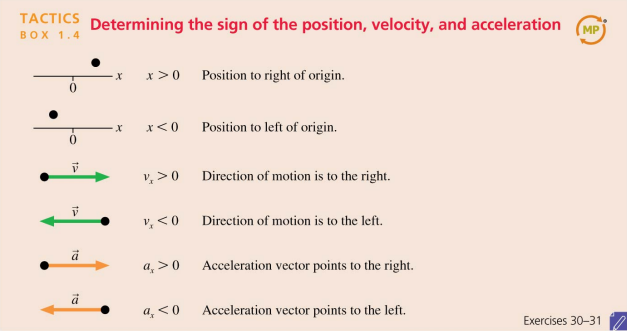
\includegraphics[width=\textwidth]{../figures/tactics1_4.png}
\end{center}
\begin{itemize}
   \item The sign of acceleration tells us which way the acceleration vector points, {\bf NOT} whether the object is speeding up or slowing down.
\end{itemize}
\end{frame}

\begin{frame}{1D Motion}
\begin{center}
   Slowing down (dwn) or speeding up (up)? Do you see a pattern?\\~\\
\begin{tabular}{ c|c|c }
   Velocity & Acceleration & dwn/up \\
   \hline
   {\large +} &  {\large +} & \uncover<2>{up} \\ 
   \hline
   {\large -} &  {\large +} & \uncover<3>{dwn} \\ 
   \hline
   {\large +} &  {\large -} & \uncover<4>{dwn} \\ 
   \hline
   {\large -} &  {\large -} & \uncover<5>{up} \\ 
\end{tabular}
\end{center}
\uncover<6>{~\\Pattern: Same sign means speeding up, oppositite means slowing down.}
\end{frame}

\begin{frame}{1D Motion - Quick Check}
\begin{center}
   A cyclist riding at 20 mph sees a stop sign and actually comes to a complete stop in 4 s. He then, in 6 s, returns to a speed of 15 mph. Which is his motion diagram? (Just think about what we just talked about)
   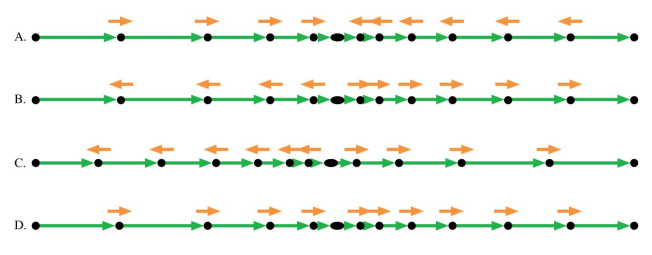
\includegraphics[width=\textwidth]{../figures/QC1_6.png}
   \only<2->{\checkh{0.7cm}{4.8cm}}
\end{center}
\end{frame}

\begin{frame}{1D Motion - Quick Check}
\begin{center}
   An X-wing (not the USS Enterprise) is traveling to the left and is slowing down in preparation for his attack run on the Death Star. The coordinate system is\\ $\rightarrow +x$\\ The velocity and acceleration are\\~\\
\begin{enumerate}[A.]
   \item Velocity is positive, acceleration is positive.
   \item Velocity is negative, acceleration is positive.
   \item Velocity is positive, acceleration is negative.
   \item Velocity is negative, acceleration is negative.
\end{enumerate}
   \only<2->{\checkh{0.5cm}{5.3cm}}
\end{center}
\end{frame}

\begin{frame}{1D Motion}
\begin{itemize}
   \item Another useful tool (in addition to a motion diagram) is an x vs. t graph, like the ones you are generating in lab. Let's see if you are able to convert this motion diagram into an x vs. t graph. \\~\\
\end{itemize}
\begin{center}
   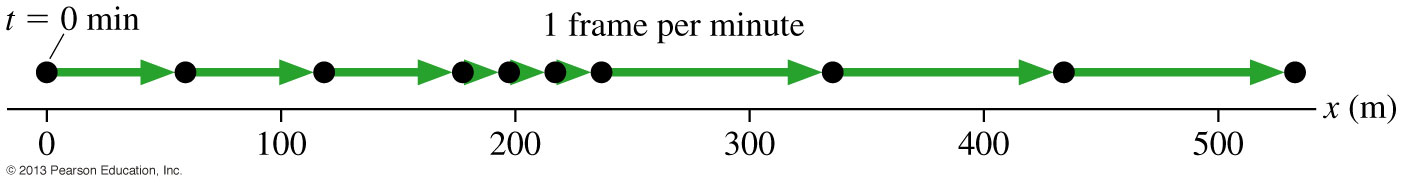
\includegraphics[width=\textwidth]{../figures/01_20_Figure.jpg}
   \\~\\ \uncover<2>{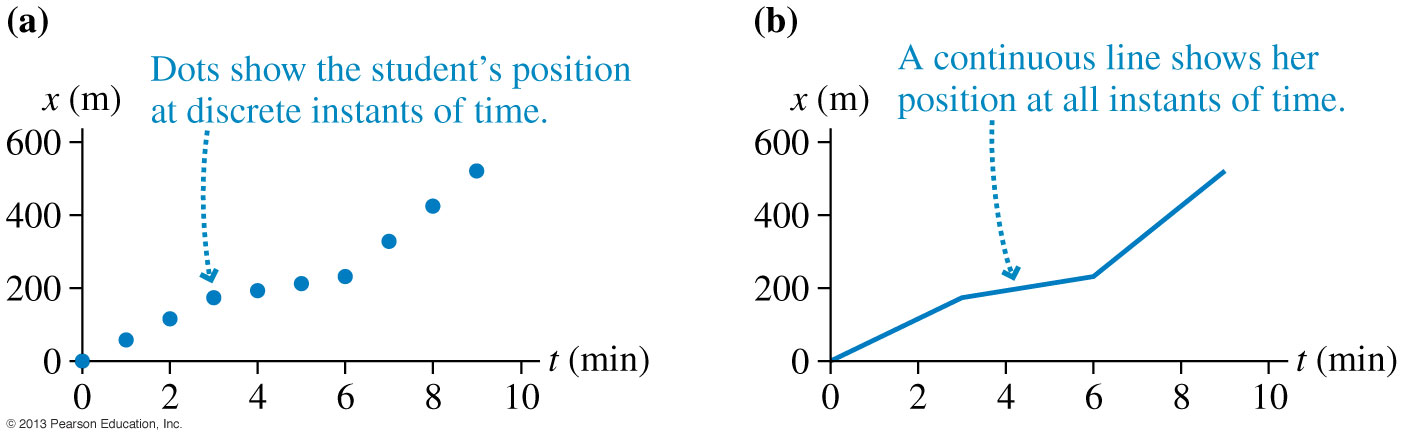
\includegraphics[width=\textwidth]{../figures/01_21_Figure.jpg}}
\end{center}
\end{frame}

\begin{frame}{1D Motion}
\begin{center}
   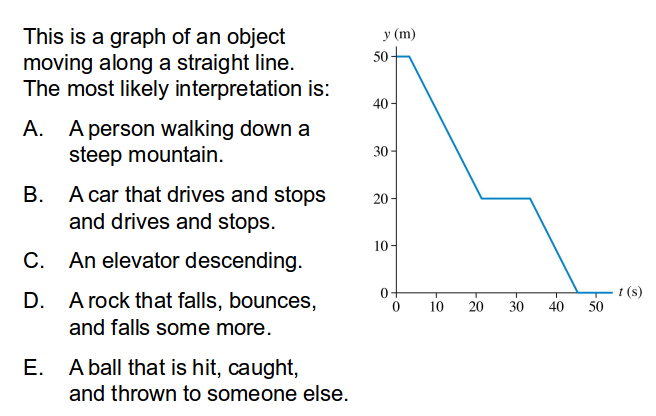
\includegraphics[width=\textwidth]{../figures/QC1_10.png}
   \only<2->{\checkH{0.8cm}{5.0cm}}
\end{center}
\end{frame}

\begin{frame}{Uniform Motion}
\begin{itemize}
   \item {\bf Uniform Motion} is motion in which each each successive equal-time interval has the same displacement. This is a subset of 1D motion. You can only have motion in a straight line, but also you don't change velocity (speed or direction).
   \item For example, if you drive your car at a perfectly steady 60 mph, this means you change your position by 60 miles for every time interval of 1 hour.
   \begin{equation*}
      v_{ave} = \frac{\Delta x}{\Delta t}
   \end{equation*}
\end{itemize}
\end{frame}

\begin{frame}{Uniform Motion}
\begin{itemize}
   \item<1-> What would uniform motion look like on a graph?
   \item<1-> How would you find the velocity of an object with uniform motion from a graph?\\~\\
\end{itemize}
\begin{center}
   \uncover<2>{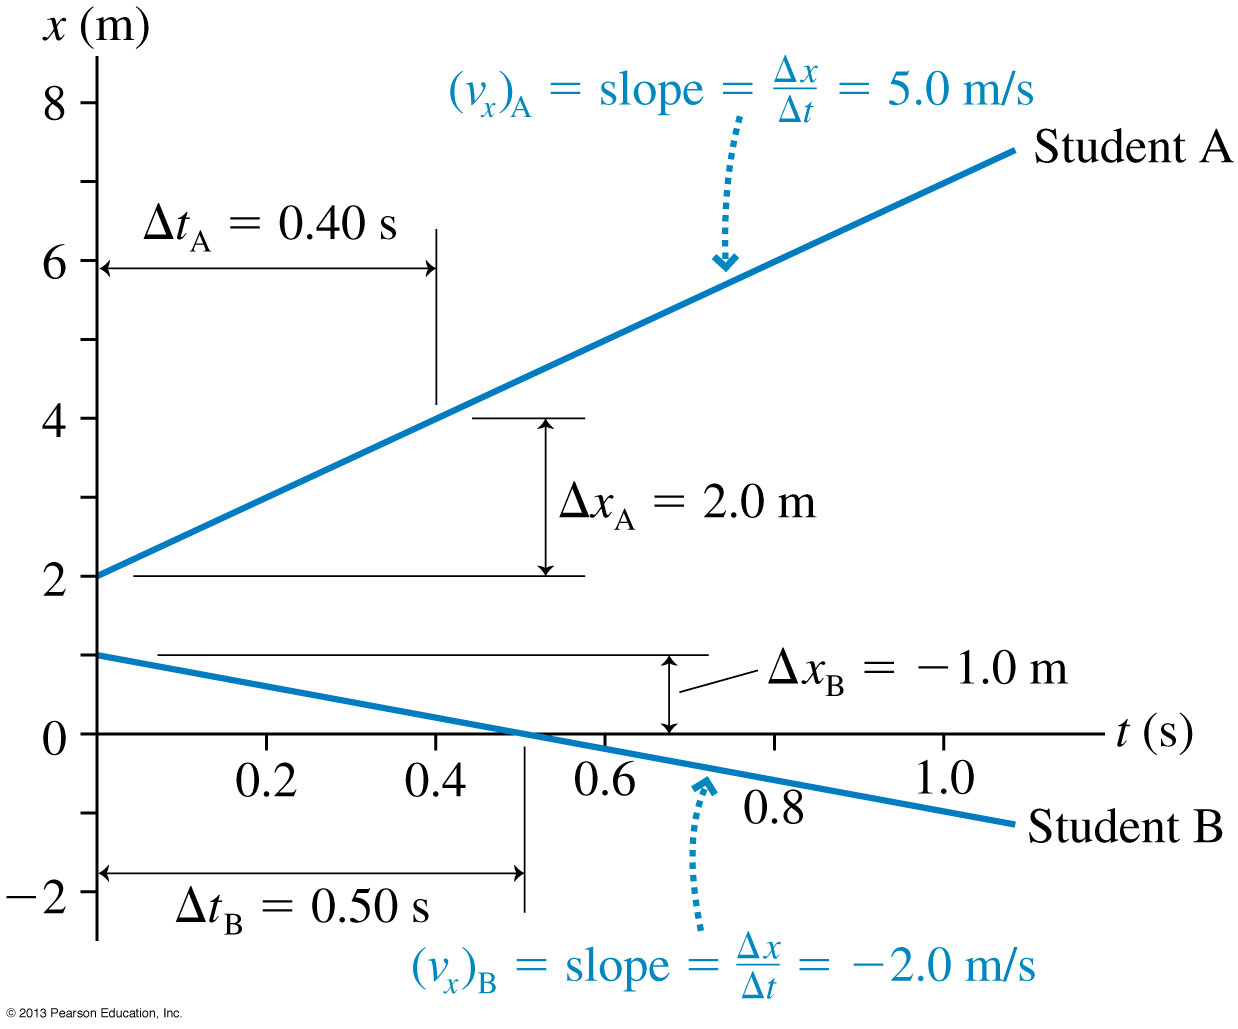
\includegraphics[width=0.6\textwidth]{../figures/02_02_Figure.jpg}}
\end{center}
\end{frame}

\begin{frame}{Uniform Motion}
\begin{itemize}
   \item It turns out that the slope of the position vs. time graph is the velocity (We'll talk about this in terms of derivatives next time but since this is a constant slope it doesn't matter right now).
\uncover<2>{
   \begin{columns}
   \begin{column}{0.5\textwidth}
      \begin{center}
         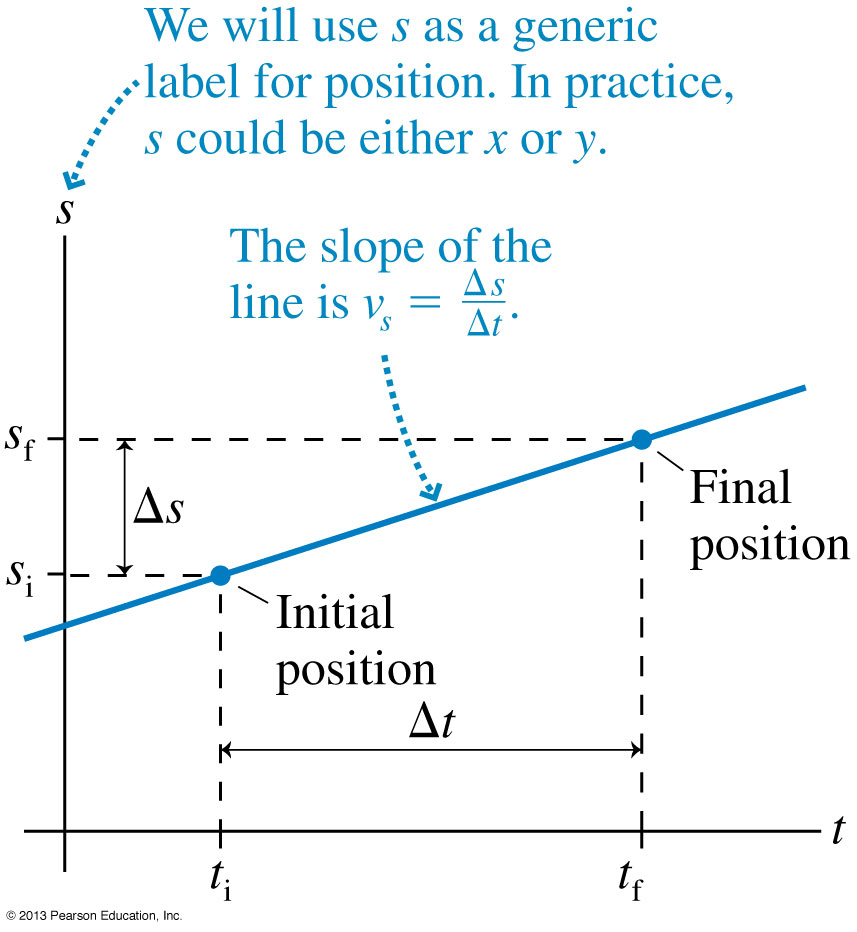
\includegraphics[width=0.5\textwidth]{../figures/02_03_Figure.jpg}
      \end{center}
   \end{column}
   \begin{column}{0.5\textwidth}
      If the position of a particle is given by $s$ and the velocity is the slope then we can write
      \begin{equation*}
         v_s = \frac{\mathrm{rise}}{\mathrm{run}} = \frac{\Delta s}{\Delta t} = \frac{s_f-s_i}{t_f-t_i}
      \end{equation*}
   \end{column}
   \end{columns}
}
\end{itemize}
\uncover<3>{
\vspace{0.7cm}
\begin{shaded}
\begin{equation}
   s_f = s_i + v_s\Delta t ~~~~~\mathrm{(Uniform Motion Equation)}
\end{equation}
\end{shaded}
}
\end{frame}

\begin{frame}{Problem Solving Strategy}
\begin{enumerate}
   \item {\bf Draw a motion diagram:} This developes intuition/visualize of the motion.
   \item {\bf Establish a coordinate system:} Choose an axis and origin that seem ``good" for the motion.
   \item {\bf Sketch the situation:} Show the object at the beginning and end of the motion, and at any point where the motion changes in the middle.
   \item {\bf Define symbols:} Place the symbols at relevant places on the sketch.
   \item {\bf List known information:} Make a table of quantities that you know, or that are easily found out.
   \item {\bf Identify the desired unknowns:} Make a table of quantities that you need to find to solve the problem.
\end{enumerate}
\end{frame}

\begin{frame}{Uniform Motion Example using the problem solving strategy}
\begin{center}
   An hocker player is on a break away headed toward the other teams goal. He travels the whole time at 10 m/s. He is currently in the middle of the two goals which are about 52 m apart. How long does the goalie have to prepare for the shot? (Assume he shoots right as he gets to the goal)
   \begin{columns}
   \begin{column}{0.4\textwidth}
      \begin{center}
         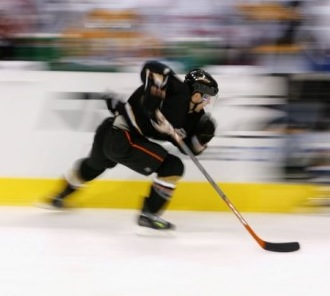
\includegraphics[width=\textwidth]{../figures/hockey1.jpg}
      \end{center}
   \end{column}
   \begin{column}{0.6\textwidth}
   \begin{enumerate}
      \item Draw a motion diagram
      \item Establish a coordinate system
      \item Sketch the situation
      \item Define symbols
      \item List known information
      \item Identify the desired unknowns
   \end{enumerate}
   \end{column}
   \end{columns}
   \uncover<2>{\red{$t=2.6$ s}}
\end{center}
\end{frame}

\begin{frame}{Uniform Motion Example using the problem solving strategy}
\begin{center}
   Two billiard balls, labeled 1 and 2, are initially at rest on a smooth pool table and are separated by a distance of 50.0 m. Simultaneously, each ball is given a quick hit, and they begin to roll directly toward each other. Ball 1 moves with a speed of 5.23 m/s , and ball 2 moves with a speed of 2.67 m/s.
What is the distance covered by ball 1 by the time the two balls collide? \\~\\
   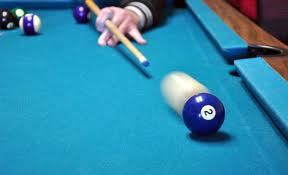
\includegraphics[width=0.6\textwidth]{../figures/billiard-balls1.jpg}
\end{center}
\end{frame}

\begin{frame}{Picture References}
\tiny
Hockey Player, accessed 28 Aug 2017: \href{http://www.kevinneeld.com/breakaway-hockey-speed-qa/}{http://www.kevinneeld.com/breakaway-hockey-speed-qa/}\\
Billiard Balls, accessed 28 Aug 2017: \href{http://www.healingtalks.com/wp-content/uploads/2011/12/billiard-balls.jpg}{http://www.healingtalks.com/wp-content/uploads/2011/12/billiard-balls.jpg}
\end{frame}

\end{document}
